% Dies ist eine Vorlage für Eure Bachelorarbeit an der RUB,
% erstellt von Alexander Noack, zur freien Verwendung ;-)

\RequirePackage[l2tabu,orthodox]{nag} % checke common mistakes/outdated pkgs
% Die KOMA Klasse für article mit einer 11pt Schrift auf A4 Papier
\documentclass[11pt,
               a4paper,
               parskip=half, style=authoryear, citestyle=authoryear-comp
              bibliography=totoc,
               ]{scrartcl}

% ============ %
% Pakete laden %
% ============ %
\newcommand{\dif}[2][]{$d^{#1} {#2}$} 
\newcommand{\todoo}[1]{\textcolor{red}{#1}} 

\usepackage[backend=bibtex,style=authoryear,
natbib=true]{biblatex}

\bibliography{name.bib}




\usepackage[colorinlistoftodos,prependcaption,textsize=tiny]{todonotes}
\usepackage[disable]{todonotes}

\usepackage{lipsum}
\usepackage{caption}
\usepackage{subcaption}
\usepackage[disable]{todonotes}
\usepackage[ngerman=ngerman-x-latest]{hyphsubst} % als erstes laden!

% Input encoding auf utf8 setzen, und die Ausgabe in T1 kodieren (Westeuropa)
\usepackage[utf8]{inputenc} % in einer aktuellen LaTeX Version nicht nötig
\usepackage[T1]{fontenc}

% geometry -- praktisch, wenn man genaue Vorstellungen/Vorgaben des Layouts hat
\usepackage[pass]{geometry} % Option pass übergibt die Werte von KOMA

% Kopf- und Fußzeile verändern
\usepackage{scrlayer-scrpage}

% Nutze latin modern font und fixe ein paar Probleme
\usepackage{lmodern}
\usepackage{fixcmex}

% Mikro-Typographie
\usepackage{microtype}

% Deutsche Sprache mit _n_euer Rechtschreibung zusätzlich zu englisch
\usepackage[english,ngerman]{babel}

% Komfortables Titel-, Autor-, .. -Handling
\usepackage{titling}

% Um zum Beispiel Grafiken einzubinden
\usepackage[usenames,dvipsnames]{xcolor}
\usepackage{graphicx} % lädt auch xcolor 

% Mathematik Pakete und extra Symbole
%\usepackage{amsmath}
\usepackage{mathtools} % lädt auch amsmath
\usepackage{amssymb}
\usepackage{textcomp}
\usepackage{gensymb}

% Ermöglicht komfortabel das Anpassen von Abständen, Labels etc. für itemize
\usepackage{enumitem}

% Für mehrere Bilder die zusammengehören praktisch
\usepackage{subcaption}

% Lade Tabellen Pakete
\usepackage{array}
\usepackage{booktabs}
\usepackage{multirow}
%\usepackage{tabularx}
%\usepackage{longtable}
\usepackage{csvsimple}

% Um Quellcode einzubinden
\usepackage{listings}

% Um mit LaTeX zu zeichnen und zu plotten
%\usepackage{tikz}
%\usepackage{pgfplots} % lädt auch tikz

% Physik- und formel- oder symbolbezogene Pakete
\usepackage{siunitx}
\usepackage{physics}
%\usepackage{braket}
\usepackage[thinc]{esdiff}

% Erleichtern das Leben beim Editieren, Probelesen und Arbeiten
\usepackage{blindtext}
\usepackage[colorinlistoftodos]{todonotes}
\usepackage{lineno}

% Paket für wörtliche Zitate, URLs, einstellbaren Zeilenabstand
\usepackage{csquotes}
\usepackage{url}
\usepackage{setspace}

% Pakete, um User-defined-Macros zu erstellen, oder vorhandene zu verändern
\usepackage{xspace}
%\usepackage{xparse}

% für anklickbare Links (cross-referencing) ins Dokument und nach außen.
\usepackage[hidelinks,
            linktocpage=false,
            pdfusetitle]{hyperref} % als letztes (spät, exceptions) laden!
\usepackage{bookmark} % als letzteres laden, Optimierungen zu hyperref, \pdfbookmark

% =============== %
% Ende für Pakete %
% =============== %


% User-defined macros
\newcommand{\zB}{z.\,B.\xspace}
\newcommand{\ZB}{Z.\,B.\xspace}
\newcommand{\textsw}[1]{\texttt{#1}} % sw=software
\newcommand{\file}[1]{\texttt{#1}} % file names

% Header, Footer
\ihead{\thetitle} % inner head (einseitig links)
\chead{} % center head
\ohead{\rightmark} % outer head (einseitig rechts)
\automark{section} % setze \rightmark auf section name
\automark*{subsection} % falls subsection vorhanden auf diese
\setkomafont{pagehead}{\sffamily} % Kopfzeilen-Font

% list related (itemize, enumerate)
\setlist{nosep} % entferne alle Abstände
\setitemize[1]{label=\raisebox{.37ex}{\scalebox{.6}{$\bullet$}}} % kleinere bullet

% math related
\AtBeginDocument{% verkleinere Raum um Mathe Umgebungen
  \setlength{\abovedisplayskip}{6pt plus 3pt minus 3pt}%=11pt plus 3pt minus 6pt
  \setlength{\abovedisplayshortskip}{0pt plus 3pt}%=0pt plus 3pt
  \setlength{\belowdisplayskip}{6pt plus 3pt minus 3pt}%=11pt plus 3pt minus 6pt
  \setlength{\belowdisplayshortskip}{4pt plus 3pt minus 3pt}%=6.5pt plus 3.5pt minus 3pt
}
\newcolumntype{L}{>{$}l<{$}} % math-mode version of "l" column type
\newcolumntype{C}{>{$}c<{$}} % math-mode version of "c" column type

% table related
\setlength{\cmidrulekern}{.4em}

% Neue Einheiten für siunitx
\DeclareSIUnit{\erg}{erg}
\DeclareSIUnit{\Gauss}{G}

% Titel, Autor, etc
\title{Beispieldokument EWA} % Titel in Sprache der Arbeit
\newcommand{\theothertitle}{Example Document} % Titel in anderer Sprache
\newcommand{\bachelormaster}{Bachelor} % {Bachelor} oder {Master}
\newcommand{\sciencearts}{Science} % {Science} oder {Arts}
\author{Vorname Name} % Autor
\newcommand{\placeofbirth}{Deutschland} % Geburtsort
\newcommand{\location}{Bochum}
\date{2020} % Datum (Jahr)

% ================= %
% Ende der Preamble %
%  Beginn Dokument  %
% ================= %

\begin{document}

% Titelseite
% Benötigte Pakete in dieser Version:
% geometry, hyperref, bookmark, titling, setspace
\newgeometry{margin=2.5cm,bottom=4cm}%,bindingoffset=6mm}
\pdfbookmark[section]{Titelseite}{titlepage}
\begin{titlepage}
  \centering
  {\huge\titlefont\thetitle\par
                  \bigskip\bigskip
                  \theothertitle\par}
  \vspace{2cm}

  \begin{spacing}{0.8}
    {\LARGE \bachelormaster arbeit\par
            \bigskip\medskip
            im Studiengang\par
            ,,\bachelormaster{} of \sciencearts``\par
            im Fach Physik\par
            \bigskip\medskip
            an der Fakultät für Physik und Astronomie\par
            der Ruhr-Universität Bochum\par}

    \vfill

    {\LARGE von\par
            \theauthor\par
            \bigskip\medskip
            aus\par
            \placeofbirth\par}
  \end{spacing}

  \vspace{1.8cm}

  {\LARGE \location{} \thedate\par}
\end{titlepage}
\restoregeometry
\cleardoublepage

% Table of Contents
\pdfbookmark[section]{\contentsname}{toc}
\tableofcontents
\cleardoublepage

\section{Beispieldokument}


\begin{figure}
    \centering
    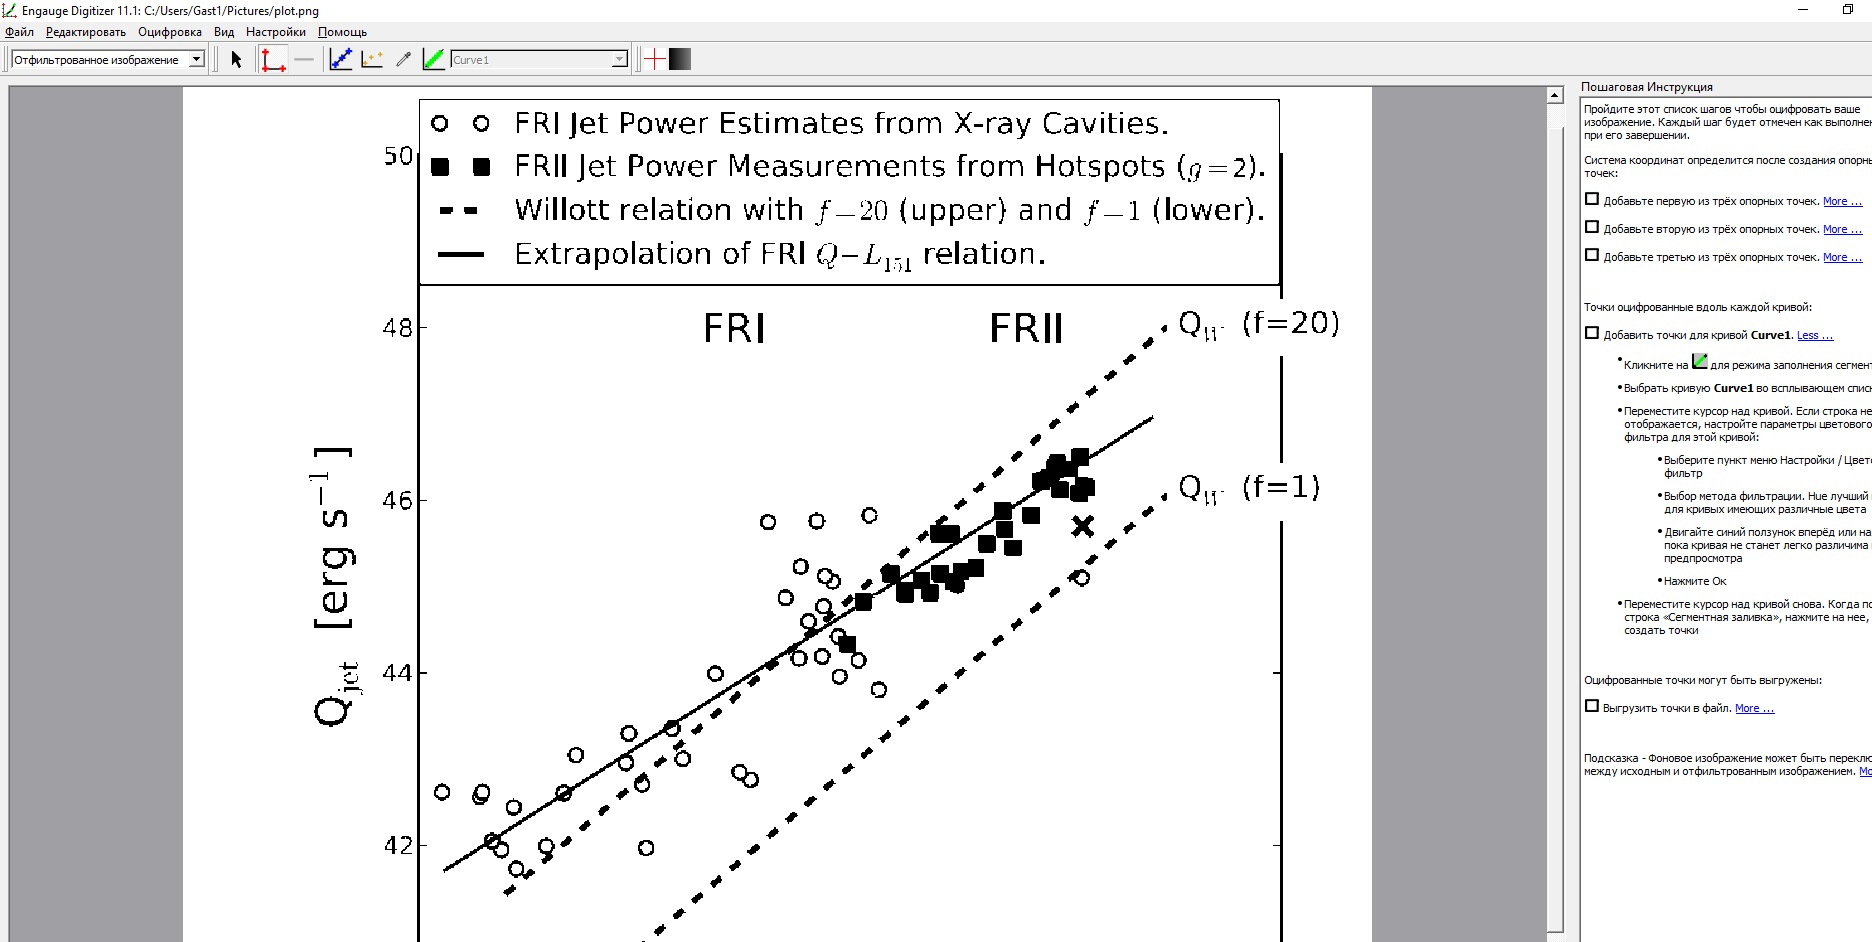
\includegraphics[scale=0.35]{shag1.jpg}
    \caption{Schritt 1: Öffnen der grafischen Datei}
    \label{fig:my_label}
\end{figure}

\begin{figure}
    \centering
    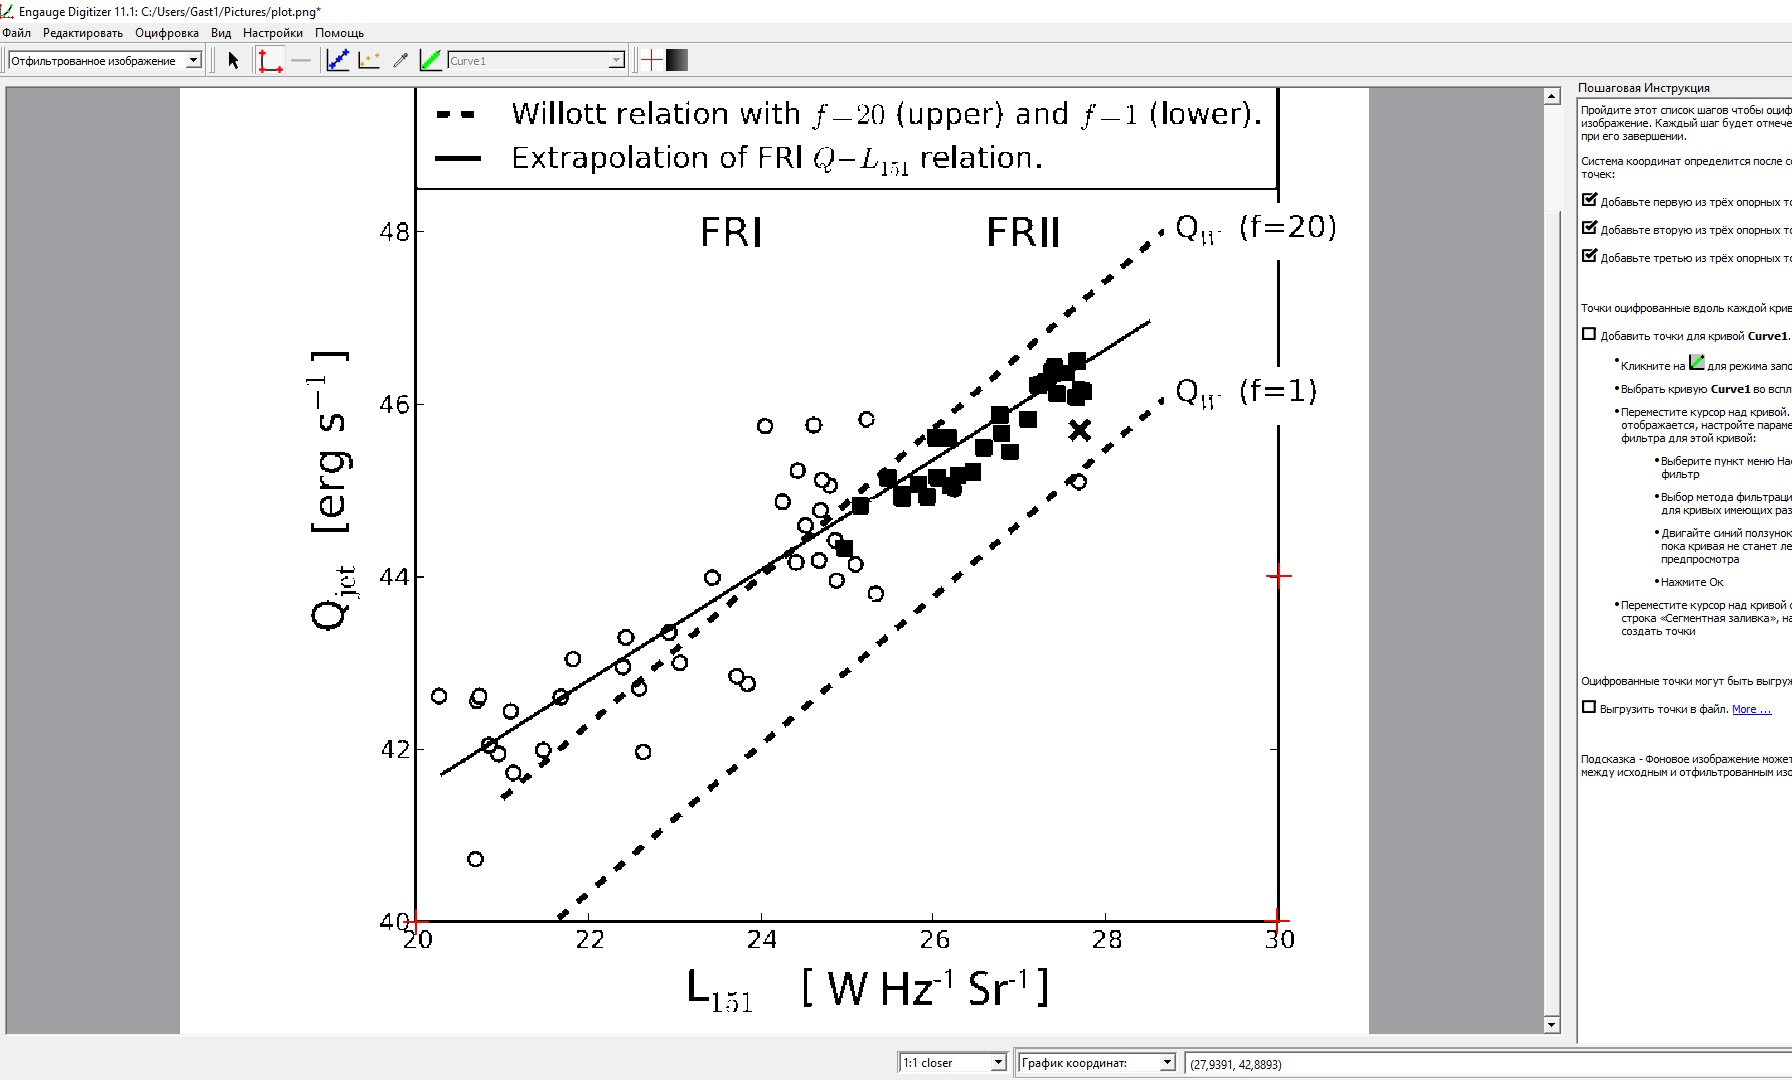
\includegraphics[scale=0.35]{shag2.jpg}
    \caption{Schritt 2: Angabe von 3 Kontrollpunkten}
    \label{fig:my_label}
\end{figure}

\begin{figure}
    \centering
    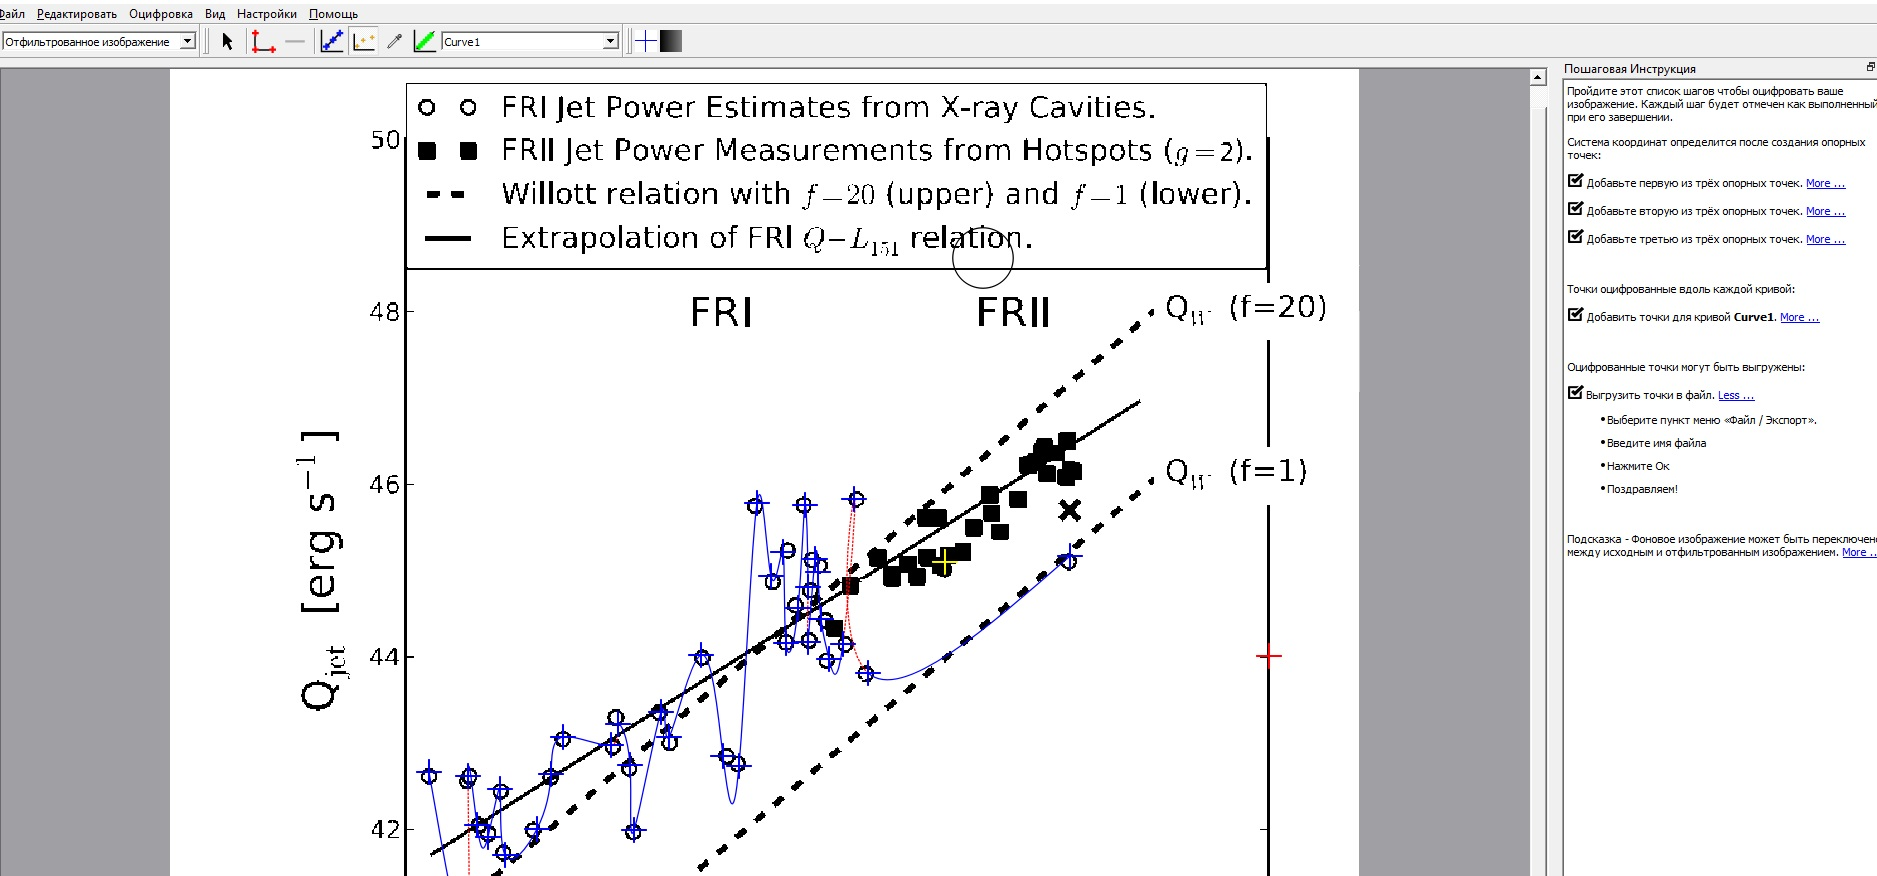
\includegraphics[scale=0.35]{shag3.jpg}
    \caption{Schritt 3: Auswählen von den ausgewerteten Punkten}
    \label{fig:my_label}
\end{figure}

\begin{table}[h]
            \centering
             \begin{tabular}{|c|c|}
               $L_{151}$ [W Hz^{-1}Sr^{-1}] & $Q_{jet} $[erg s^{-1}] \\
               \hline
              20,2585& 42,6217  \\
              \hline
              20,6864& 40,7263  \\
              \hline
              20,6907& 42,5528  \\ 
              \hline
              20,7321& 42,6218  \\
              \hline
              20,8425& 42,0559  \\
              \hline
              20,9529& 41,9455  \\
              \hline
              21,0861& 42,4424  \\
              \hline
              21,1277& 41,7247  \\
              \hline
              21,4679& 41,9915  \\
              \hline
              21,6747& 42,608  \\ 
              \hline
              21,8217& 43,0405\\
              \hline
              22,3873& 42,9532 \\
              \hline
              22,4286& 43,2982 \\
              \hline
              22,5897& 42,7047 \\
              \hline
              22,6358& 41,964\\
              \hline
              22,939& 43,3489 \\
              \hline
              23,0586& 42,9946 \\
              \hline
              23,4309& 43,9884\\
              \hline
              23,7208& 42,8428 \\
              \hline
              23,845& 42,7554\\
              \hline
              24,0426& 45,7406\\
              \hline
              24,2446& 44,8764\\
              \hline
              24,4011 & 44,1633\\
              \hline
              24,4239 & 45,2307\\
              \hline
              24,5113 & 44,5958\\
              \hline
              24,6083 & 45,7662\\
              \hline
              24,6632 & 44,1909\\
              \hline
              24,6906 & 44,7752\\
              \hline
              24,6998 & 45,1249\\
              \hline
              24,7963 & 45,0559\\
              \hline
              24,8516 & 44,4164\\
              \hline
              24,8701 & 43,9609\\
              \hline
              25,0954 & 44,1449\\
              \hline
              25,2214 & 45,8283\\
              \hline
              25,3299 & 43,8045 \\ 
              \hline
              27,6839 & 45,0975 \\
              \hline
              
      \end{tabular}
      \caption{FR I Jet power estimates from X-Ray Cavities}
       \label{tab:my_label}
        \end{table}



\end{document}
